\documentclass{beamer}

\usepackage[brazil]{babel}
\usepackage[utf8]{inputenc}
\usepackage[T1]{fontenc}
\usepackage{listings}

\usetheme{Madrid}
\setbeamertemplate{navigation symbols}{}

\lstset{
language=Python,
basicstyle=\ttfamily\tiny,
backgroundcolor=\color{white},
keywordstyle=\color{blue}\bfseries,
stringstyle=\color{red},
commentstyle=\color{green},
%morecomment=[s][\color{green}]{/**}{*/},
showspaces=false,
showstringspaces=false,
morekeywords={None,self,__init__},
literate=
{á}{{\'a}}1
{Á}{{\'A}}1
{à}{{\`a}}1 
{À}{{\`A}}1
{â}{{\^a}}1 
{Â}{{\^A}}1
{ã}{{\~a}}1
{Ã}{{\~A}}1
{ä}{{\"a}}1
{Ä}{{\"A}}1
{é}{{\'e}}1
{É}{{\'E}}1
{è}{{\`e}}1
{È}{{\`E}}1
{ê}{{\^e}}1
{Ê}{{\^E}}1
{ẽ}{{\~e}}1
{Ẽ}{{\~E}}1 
{ë}{{\"e}}1
{Ë}{{\"E}}1
{í}{{\'i}}1
{Í}{{\'I}}1
{ì}{{\`i}}1
{Ì}{{\`I}}1
{î}{{\^i}}1
{Î}{{\^I}}1
{ĩ}{{\~i}}1
{Ĩ}{{\~I}}1
{ï}{{\"i}}1
{Ï}{{\"I}}1
{ó}{{\'o}}1
{Ó}{{\'O}}1
{ò}{{\`o}}1
{Ò}{{\`O}}1
{ô}{{\^o}}1
{Ô}{{\^O}}1
{õ}{{\~o}}1
{Õ}{{\~O}}1
{ö}{{\"o}}1
{Ö}{{\"O}}1
{ú}{{\'u}}1
{Ú}{{\'U}}1
{ù}{{\`u}}1
{Ù}{{\`U}}1
{û}{{\^u}}1
{Û}{{\^U}}1
{ũ}{{\~u}}1
{Ũ}{{\~U}}1
{ü}{{\"u}}1
{Ü}{{\"U}}1
{ç}{{\c{c}}}1
{Ç}{{\c{C}}}1
}

\title[Programação Orientada a Objetos]{Programação Orientada a Objetos em Python}

\author[Diego S. C. Nascimento]{Diego Silveira Costa Nascimento}

\institute[IFRN]{
Instituto Federal de Educação, Ciência e Tecnologia do Rio Grande do Norte\\
diego.nascimento@ifrn.edu.br
}

\date[\today]{\today}

\begin{document}

\begin{frame}[plain]
	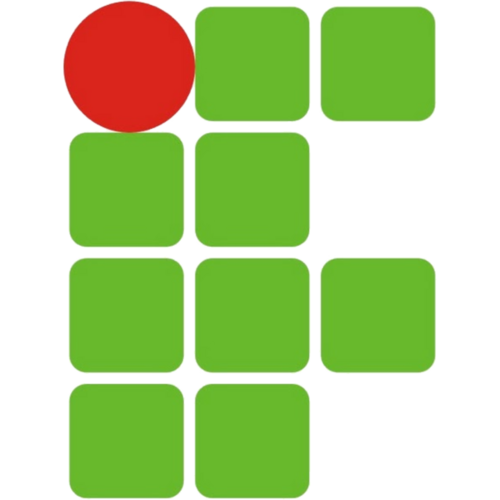
\includegraphics[scale=0.2]{./imagens/IFRN}
	\titlepage
\end{frame}

\logo{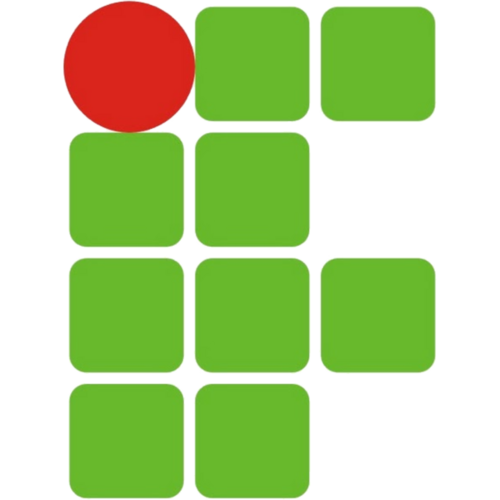
\includegraphics[scale=0.1]{./imagens/IFRN}}

\begin{frame}
	\frametitle{Ementa do Curso}
  	\tableofcontents
\end{frame}

\AtBeginSection[]{
	\begin{frame}
		\frametitle{Ementa do Curso}
		\tableofcontents[currentsection]
	\end{frame}
}

\section{Introdução}

\begin{frame}
	\frametitle{Motivações}
	
	\begin{itemize}
		\item O desenvolvimento de aplicações de software estão cada vez mais complexas;
        \item Cresceram as demandas por metodologias que pudessem abstrair e modularizar as estruturas básicas de programas; e
        \item A maioria das linguagens de programação suportam orientação a objetos: Haskell, Java, C++, Python, PHP, Ruby, Pascal, entre outras.
	\end{itemize}
\end{frame}

\begin{frame}
	\frametitle{História}
	
	\begin{itemize}
		\item Em 1967, Kristen Nygaard e Ole-Johan Dahl, do Centro Norueguês de Computação em Oslo, desenvolveram a linguagem Simula 67 que introduzia os primeiros conceitos de orientação a objetos;
		\item Em 1970, Alan Kay, Dan Ingalls e Adele Goldberg, do Centro de Pesquisa da Xerox, desenvolveram a linguagem totalmente orientada a objetos;

		\item Em 1979--1983, Bjarne Stroustrup, no laboratório da AT \& T, desenvolveu a linguagem de programação C++, uma evolução da linguagem C; e
		
		\item Maior  divulgação  a  partir  de  1986  no primeiro workshop ``Object-Oriented  Programming  Languages, Systems  and  Applications''.
	\end{itemize}
\end{frame}

\begin{frame}
	\frametitle{Principais Vantagens}
	
	\begin{itemize}
		\item Aumento de produtividade;
		\item Reúso de código;
		\item Redução das linhas de código programadas;
		\item Separação de responsabilidades;
		\item Componentização;
		\item Maior flexibilidade do sistema; e
		\item Facilidade na manutenção.
	\end{itemize}
\end{frame}

\begin{frame}
	\frametitle{Objetos}
	
	\begin{itemize}
		\item É a metáfora para se compreender a tecnologia orientada a objetos;
		\item Estamos rodeados por objetos: mesa, carro, livro, pessoa, etc; e
		\item Os objetos do mundo real têm duas características em comum:
		\begin{itemize}
			\item Estado -- representa as propriedades (nome, peso, altura, cor, etc.); e
			\item Comportamento -- representa ações (andar, falar, calcular, etc.).
		\end{itemize}
	\end{itemize} \vfill
	
	\begin{exampleblock}{Ilustações}
		\begin{center}
			
\includegraphics[scale=0.3]{./imagens/carro}~~~
			
\includegraphics[scale=0.3]{./imagens/celular}~~~
			
\includegraphics[scale=0.3]{./imagens/pessoa}
		\end{center}
	\end{exampleblock}
\end{frame}


\begin{frame}
	\frametitle{Orientação a Objetos}

	\begin{block}{Definição}
		É um paradigma para o desenvolvimento de software que basea-se na utilização de componentes individuais (objetos) que colaboram para construir sistemas mais complexos. 
	\end{block}\vfill
	
	\begin{itemize}
	  \item A colaboração entre os objetos é feita através do envio de mensagens;
	  \item Descreve uma série de técnicas para estruturar soluções para problemas
	  computacionais; e
	  \item É um paradigma de programação no qual um programa é estruturado em
	  objetos.
	\end{itemize}
\end{frame}

\begin{frame}
	\frametitle{Os Quatros Pilares}
	
	\begin{enumerate}
	   \item Abstração;
	   \item Encapsulamento;
	   \item Herança; e
	  \item Polimorfismo.
	\end{enumerate}
\end{frame}

\section{Abstração}

\begin{frame}
	\frametitle{Classes}
	
	\begin{itemize}
	  \item A estrutura fundamental para definir novos objetos é a classe; e
	  \item Uma classe é definida em código-fonte.
	\end{itemize} \vfill
	
	\begin{exampleblock}{Ilustração}
		\begin{center}
			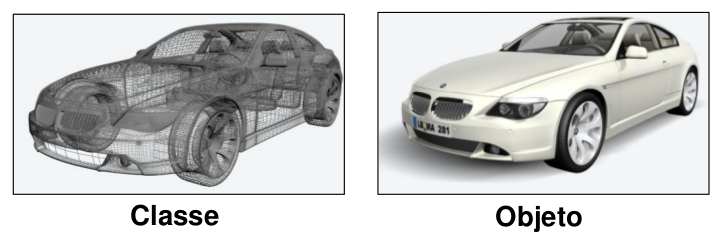
\includegraphics[scale=0.3]{./imagens/classe-objeto}
		\end{center}		
	\end{exampleblock}
\end{frame}

\begin{frame}
	\frametitle{Classe em Python}
		
	\begin{block}{Estrutura}
		\textbf{class} nome\_da\_classe:\\
		~~~~atributos\\
		~~~~construtor\\
		~~~~métodos
	\end{block}
\end{frame}

\begin{frame}[fragile]
	\frametitle{Demonstração de Classe}
	
	\begin{exampleblock}{Exemplo}
		\begin{lstlisting}
class Conta:		
    numero = None
    saldo = None
		\end{lstlisting}
	\end{exampleblock}
\end{frame}

\begin{frame}
	\frametitle{Instância}
	
	\begin{itemize}
	  \item Uma instância é um objeto criado com base em uma classe definida;
	  \item Classe é apenas uma estrutura, que especifica objetos, mas que não
	  pode ser utilizada diretamente;
	  \item Instância representa o objeto concretizado a partir de uma classe;
	  \item Uma instância possui um ciclo de vida:
	  \begin{itemize}
	    \item Criada;
	    \item Manipulada; e
	    \item Destruída. 
	  \end{itemize}
	\end{itemize} \vfill
	
	\begin{block}{Estrutura}
		variável = \textbf{Classe()}
	\end{block}
\end{frame}

\begin{frame}[fragile]
	\frametitle{Demonstração de Instância}
	
	\begin{exampleblock}{Exemplo}
		\begin{lstlisting}
conta = Conta()
conta.numero = 1
conta.saldo = 10
print(conta.numero)
print(conta.saldo)
        \end{lstlisting}
	\end{exampleblock}
\end{frame}

\begin{frame}
	\frametitle{Construtor}
	
	\begin{itemize}
		\item Determina que ações devem ser executadas quando da criação de um objeto; e
		\item Pode possuir ou não parâmetros.
	\end{itemize} \vfill
	
	\begin{block}{Estrutura}
	\textbf{def} \_\_\textbf{init}\_\_(\textbf{self},parâmetros):
	\end{block}
\end{frame}

\begin{frame}[fragile]
	\frametitle{Demonstração de Construtor}
	
	\begin{exampleblock}{Exemplo}
		\begin{lstlisting}
class Conta:
    def __init__(self,numero):
        self.numero = numero
        self.saldo = 0.0
			    			   			
conta = Conta(1)	
print(conta.numero)
print(conta.saldo)
		\end{lstlisting}
	\end{exampleblock}
\end{frame}


\begin{frame}
	\frametitle{Métodos}
	
	\begin{itemize}
		\item Representam os comportamentos de uma classe;
		\item Premitem que acessemos os atributos, tanto para recuperar os valores, como para alterá-los caso necessário;
		\item Podem retornam ou não algum valor; e
		\item Podem possuir ou não parâmetros.
	\end{itemize} \vfill 
	
	\begin{block}{Estrutura}
		\textbf{def} nome\_do\_método(\textbf{self},parâmetros):
	\end{block} \vfill
	
	\begin{alertblock}{Importante}
		O parâmetro \textbf{self} é obrigatório.
	\end{alertblock}
\end{frame}

\begin{frame}[fragile]
	\frametitle{Demonstração de Métodos}
	
	\begin{exampleblock}{Exemplo}
		\begin{lstlisting}
class Conta:
    def __init__(self,numero):
        self.numero = numero
        self.saldo = 0.0

    def consultar_saldo(self):
        return self.saldo

    def creditar(self,valor):
        self.saldo += valor

    def debitar(self,valor):
        self.saldo -= valor

    def transferir(self,conta,valor):
        self.saldo -= valor
        conta.saldo += valor

conta1 = Conta(1)
conta1.creditar(10)
conta2 = Conta(2)
conta2.creditar(5)
print(conta1.consultar_saldo())
print(conta2.consultar_saldo())
conta1.transferir(conta2,5)
print(conta1.consultar_saldo())
print(conta2.consultar_saldo())
		\end{lstlisting}
	\end{exampleblock}
\end{frame}

\section{Encapsulamento}

\begin{frame}
	\frametitle{Encapsulamento}
	
	\begin{itemize}
	  \item Consiste em separar os aspectos externos de um objeto dos detalhes
	  internos de implementação;
	  \item Evita que dados específicos de uma aplicação possa ser acessado
	  diretamente; e
	  \item Protege os atributos ou métodos de uma classe.
	\end{itemize} \vfill
	
	\begin{exampleblock}{Ilustração}
		\begin{center}
			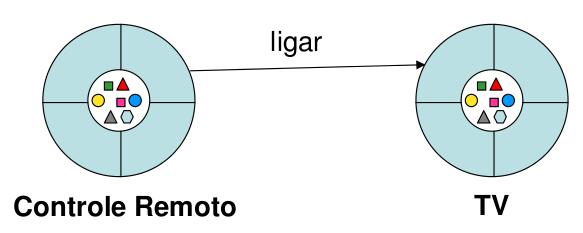
\includegraphics[scale=0.3]{./imagens/encapsulamento}
		\end{center}		
	\end{exampleblock}
\end{frame}

\begin{frame}
	\frametitle{Modificadores de Acesso}
	
	\begin{itemize}
	  \item Em Python, existem dois tipos de modificadores de acesso para atributos
	  e métodos:
	  \begin{itemize}
	    \item Público; ou
	    \item Privado.
	  \end{itemize}
	  \item Atributos ou métodos iniciados por dois sublinhados são privados e
	  todas as outras formas são públicas.
	\end{itemize}
\end{frame}

\begin{frame}[fragile]
	\frametitle{Demonstração de Encapsulamento}
	
	\begin{exampleblock}{Exemplo}
		\begin{lstlisting}
class Conta:
    def __init__(self, numero):
        self.__numero = numero
        self.__saldo = 0.0

    def consultar_saldo(self):
        return self.__saldo

    def creditar(self, valor):
        self.__saldo += valor

    def debitar(self, valor):
        self.__saldo -= valor

    def transferir(self, conta, valor):
        self.__saldo -= valor
        conta.__saldo += valor

conta = Conta(1)
conta.creditar(100)
conta.__saldo = 200.0 #Não é possível alterar o saldo da conta

print(conta.consultar_saldo())
        \end{lstlisting}
	\end{exampleblock}
\end{frame}

\section{Herança}

\begin{frame}
	\frametitle{Herança}
	
	\begin{itemize}
	  \item É uma forma de abstração utilizada na orientação a objetos;
	  \item Pode ser vista como um nível de abstração acima da encontrada entre
	  classes e objetos;
	  \item Na herança, classes semelhantes são agrupadas em hierarquias;
	  \item Cada nível de uma hierarquia pode ser visto como um nível de abstração;
	  \item Cada classe em um nível da hierarquia herda as características das
	  classes nos níveis acima;
	  \item É uma forma simples de promover reuso através de uma generalização;
	  \item Facilita o compartilhamento de comportamento comum entre um conjunto de
	  classes semelhantes; e
	  \item As diferenças ou variações de uma classe em particular podem ser
	  organizadas de forma mais clara.
	\end{itemize}
\end{frame}

\begin{frame}
	\frametitle{Herança}
	
	\begin{block}{Estrutura}
	\textbf{class}
	nome\_da\_classe(classe\_pai\_1, classe\_pai\_2, classe\_pai\_n):\\
	~~~~atributos\\
	~~~~métodos
	\end{block}\vfill	
\end{frame}

\begin{frame}[fragile]
	\frametitle{Demonstração de Herança}
		
	\begin{exampleblock}{Exemplo}
		\begin{lstlisting}
class Poupanca(Conta):
    def __init__(self,numero):
        super().__init__(numero)
        self.__rendimento = 0.0
    
    def consultar_rendimento(self):
        return self.__rendimento

    def gerar_rendimento(self,taxa):
        self.__rendimento += super().consultar_saldo() * taxa / 100

conta = Poupanca(1)
conta.creditar(200.0)
conta.gerar_rendimento(10)
print(conta.consultar_saldo())
print(conta.consultar_rendimento())        
       \end{lstlisting}
	\end{exampleblock}
\end{frame}

\section{Polimorfismo}

\begin{frame}
	\frametitle{Polimorfismo}
	
	\begin{itemize}
	  \item É originário do grego e significa ``muitas formas'' (poli = muitas,
	  morphos = formas);
	  \item Indica a capacidade de abstrair várias implementações diferentes em uma
	  única interface;
	  \item É o princípio pelo qual duas ou mais classes derivadas de uma mesma
	  superclasse podem invocar métodos que têm a mesma identificação (assinatura)
	  mas comportamentos distintos; e
	  \item Quando polimorfismo está sendo utilizado, o comportamento que será
	  adotado por um método só será definido durante a execução.
	\end{itemize}
\end{frame}

\begin{frame}[fragile]
	\frametitle{Demonstração de Polimorfismo}
		
	\begin{exampleblock}{Exemplo}
	   \begin{lstlisting}
class Poupanca(Conta):
    def __init__(self,numero):
        super().__init__(numero)
        self.__rendimento = 0.0
    
    def consultar_rendimento(self):
        return self.__rendimento

    def gerar_rendimento(self,taxa):
        self.__rendimento += super().consultar_saldo() * taxa / 100

    def consultar_saldo(self):
        return super().consultar_saldo() + self.__rendimento

conta = Poupanca(1)
conta.creditar(200.0)
conta.gerar_rendimento(5)
print(conta.consultar_saldo())
       \end{lstlisting}
	\end{exampleblock}
\end{frame}

\end{document}